\chapter{Двухчастотное волновое смешение в импульсном режиме}\label{ch: q_mixing}

В данной главе будут описаны эффекты волнового смешения, возникающие при импульсной бихроматической накачке двухуровневой системы. В этих экспериментах на кубит подаются последовательности прямоугольных или близких к ним по форме импульсов. Несущие частоты этих последовательностей незначительно отстроены от резонанса кубита, длительности импульсов варьируются от $0$ до нескольких $T_1$ кубита, а промежутки между импульсами значительно превышают $T_1$. Качественная картина спектра эластичного рассеяния претерпевает значительные изменения по сравнению с непрерывной накачкой. Например, при рассеянии синхронизированных прямоугольных импульсов на частотах $\omega_{pm}$ наблюдается бесселевская динамика боковых компонент сигнала в зависимости от эффективной длительности импульса $\Omega\Delta t$. Совершенно новый физический эффект возникает при введении задержки между последовательностями импульсов. Длительность задержки должна превосходить длительность импульса для того, чтобы отдельные импульсы на частоте $\omega_+$ попадали на кубит раньше импульсов на частоте $\omega_-$ и не перекрывались с ними. При этом кардинально меняется вид спектра эластичного рассеяния. Вместо большого количества симметричных пиков мы наблюдаем лишь один дополнительный пик на частоте $2\omega_--\omega_+$. Этому эффекту можно дать простое качественное объяснение, напрямую вытекающее из свойства кубита поглощать не более чем единичный квант поля. В дополнение к этому, мы изучаем рассеяние последовательностей импульсов на трехуровневой эквидистантной системе, которая возникает при некотором значении внешнего магнитного потока, проходящего через петлю изучаемого нами потокового кубита. Помимо к двух компонент на исходных несущих частотах и одной компоненте от четырехволнового смешения, к эластичному спектру добавляется еще две компоненты, соотвествующие двухфотонным процессам, что подтверждает справедливость качественной интерпретации экспериментальных результатов. Последние два режима мы будем называть \textit{квантовым волновым смешением}, поскольку оно обладает рядом необычных свойств, обусловленных квантовостью сверхпроводникового искусственного атома. В дополнение к экспериментальным данным, в данном разделе проведен численный расчет спектра, согласующийся с экспериментом, а также дано строгое теоретическое обоснование трехпикового спектра рассеяния на двухуровневой системе и пятипикового спектра рассеяния на трехуровневой системе на основе формализма вторичного квантования.  
\section{Случай синхронных импульсов: бесселевская динамика}
Для изучения импульсного смешения при помощи экспериментальной схемы \ref{fig: pulse_setup_1} необходимо запрограммировать генератор импульсов произвольной формы (AWG) так, чтобы на его выходе получить последовательность прямоугольных импульсов. Несущая частота этих импульсов $\omega_{\text{IF}}/2\pi$ может варьироваться от 0 до 100 МГц, а период импульсов $T\gg 1/\Gamma_1$ обеспечивает релаксацию кубита после импульса за время, предшествующее появлению следующего импульса. Длительности импульсов $\delta t$ также меняются произвольно, технические возможности AWG позволяют получить импульсы длительностью от 2 нс и выше. Импульсный сигнал с выхода AWG попадает на квадратурный смеситель, где смешивается с сигналом локального осциллятора, приобретая таким образом несущую частоту $\omega_{d} = \omega_{\text{LO}}\pm\omega_{\text{IF}}$, где выбор знака произволен и зависит от калибровки квадратурного смесителя. Затем сигнал направляется в криостат, попадает в волновод с искусственным атомом и рассеивается на нем.  Детектирование рассеянного сигнала осуществляется при помощи спектрального анализатора либо при помощи высокоскоростного АЦП. Во втором случае на выходе сигнал испытывает обратное преобразование частоты вниз при помощи еще одного квадратурного смесителя, после чего сигнал на частоте $\omega_{\text{IF}}$ оцифровывается, а квадратуры комплексного сигнала $I$ и $Q$ вычисляются при помощи цифрового преобразования Фурье \cite{sank2014fast}.

Сгенерировав две синхронные последовательности импульсов одинаковой длительности $\Delta t_-\!=\!\Delta t_+\!=\!\Delta t$ на частотах $\omega_+$ и $\omega_-$ описанным способом и подав их на кубит, мы измеряем спектр эластичного рассеяния, усредненный по большому количествую периодов. Это достигается установлением параметра RBW (Resolution Bandwidth) спектрального анализатора до 1 кГц и ниже, что делает время усреднения более 1 мс, тогда как период следования импульсов составляет 1-10 мкс. Очевидно, что длительности $\Delta t$ импульсов оказывают ключевое влияние на характер динамики кубита, и соответственно, определяют свойства рассеянного излучения, поэтому мы снимаем зависимости интенсивностей боковых компонент от эффективной длительности импульсов $\Omega\Delta t$.
Результат этих измерений изображен на Рис \ref{fig: Bessels}. 
\begin{figure}\label{fig: Bessels}
\centering
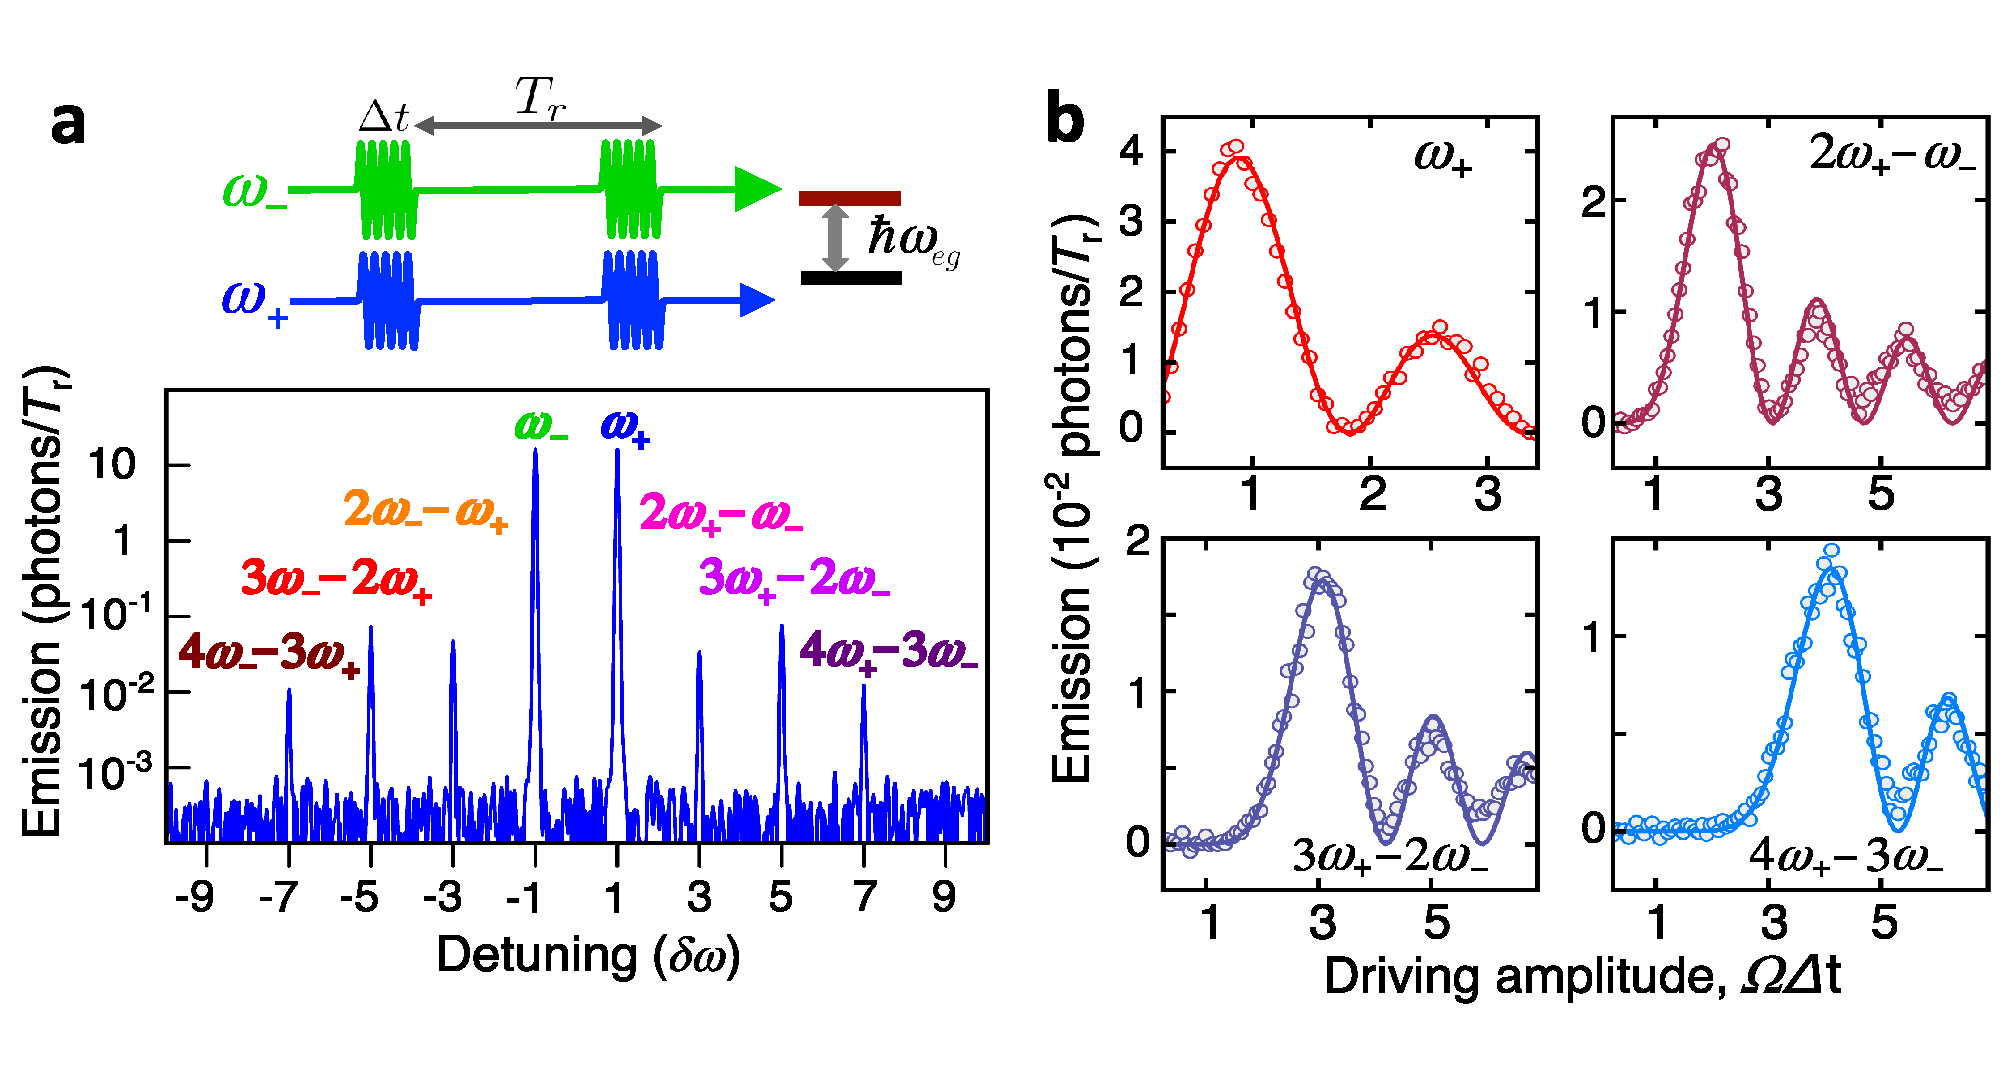
\includegraphics[width=1\textwidth]{Bessels.pdf}
\caption[Зависимость интенсивности боковых компонент от длительности импульсов $\Delta t$ бихроматической накачки]{Зависимость интенсивности боковых компонент от длительности импульсов бихроматической накачки. (a) Последовательность управляющих импульсов длительностью $\Delta t=2$~нс с периодом $T_r=1$~мкс и часть спектра эластичного рассеяния c когерентыми пиками. (б) Измеренные зависимости потока фотонов в пике от угла поворота $\zeta_{2p+1}(\Omega \Delta t). $. Точками показаны результаты измерений, сплошные линии соответствуют выражениям $J^2_{2p+1}(2\Omega\Delta t)/4$, описывающим эксперимент без подгоночных параметров.}
\end{figure} 
Этот результат достаточно просто объясняется динамикой кубита под воздействием классического поля. Для динамики кубита под действием двух классических импульсов можно получить следующее выражение:
\begin{equation}
	\braket{\sigma_-} = -\frac{1}{2}\sin(2\Omega\Delta t \cos\delta\omega t), 
\end{equation}
которое раскладывается в ряд по бесселевским функциям согласно соотношению Ангера-Якоби:
\begin{equation}
	\langle \sigma^- \rangle = -\sum_{k=-\infty}^\infty (-1)^k J_{2k+1}(2\Omega \Delta t) \cos[(2k+1)\delta\omega t],
\end{equation}
и усреднение спектральных компонент $\langle \sigma^-_{2k+1}\rangle$ с определенным набегом фазы $(2k+1)\delta \omega t$ дает:
\begin{equation}
	\langle \sigma_{2k+1}^-\rangle = \frac{(-1)^k}{2}J_{2k+1}(2\Omega t),
	\label{sclass_spectr} 
\end{equation} 
что соответствует экспериментально представленным зависимостям на Рис.~\ref{fig: Bessels}. Данный результат можно представить как разложение осцилляций Раби, которые наблюдались бы при $\delta\omega =0$, по разным спектральным компонентам.

Результат \eqref{sclass_spectr} не требует квантовомеханического описания поля, но тем не менее, мы получим его также при помощи рассмотрения эволюции кубита под воздействием двух квантованных мод поля, описывающихся операторами $a_\pm$ и $a_\pm^\dag$, взаимодействующих с кубитом. Как мы увидим далее, этот формализм позволяет описать не только случай синхронных импульсов, характеризующийся рассмотренной выше бесселевской динамикой, но и случай последовательных неперекрывающихся во времени импульсов, где спектр кардинально отличается от рассмотренного выше режима. Для начала, выпишем и обсудим несколько известных результатов для одной моды и кубита. 

Будем рассматривать двухуровневый атом с основным и возбужденными состояниями $\ket{g}$ и $\ket{e}$ и энергией $\hbar \omega_0$, взаимодействующий с квантованным полем на частоте $\omega$. Эта система может характеризоваться гамильтонианом, записанным в представлении взаимодействия:
\begin{equation}
	H = i\hbar g (a^\dag \sigma^-  e^{i\delta\omega t} - a \sigma^+  e^{-i\delta\omega t}),
	\label{Hqint}
\end{equation}
где $\hbar g$ --- энергия связи между полем и атомом, $\delta\omega = \omega - \omega_0$ --- отстройка, которую мы считаем достаточно малой, $\sigma^{+} = \ket{e}\bra{g}$ и $\sigma^{-} = \ket{g} \bra{e}$ --- повышающий и понижающий операторы для состояний атома, а $a^\dag$ ($a$) --- операторы рождения и уничтожения фотонных состояний $|n\rangle$  на частоте $\omega = \omega_0 + \delta\omega$. 
Эволюция системы на коротком временном интервале $\Delta t \ll \delta\omega^{-1}$ описывается оператором $U(t',t) = \exp(-\frac{i}{\hbar} H_t \Delta t)$, где $H_t$ --- гамильтониан в момент времени $t$, $\Delta t = t'-t$. Оператор эволюции может быть разложен в бесконечный ряд по формуле:
\begin{equation}
	\begin{split}
		U(t',t) = 1 + 
		\eta (a^\dag s^- - a s^+ ) 
		-\frac{\eta^2}{2!} (a a^{\dag} s_{e} + a^{\dag}a s_{g} ) -
		\frac{\eta^3}{3!} (a^{\dag} a a^\dag s^- - a a^{\dag}a s^+)+... ,
	\end{split}
	\label{ut}
\end{equation}
где $\eta = g\Delta t$ и $s^\pm$ --- зависящие от времени операторы $s^+(t) = \sigma^+ e^{-i\delta\omega t}$ и $s^-(t) = \sigma^- e^{i\delta\omega t}$. 
Данный ряд можно записать в более простом виде: 
\begin{equation}
	\begin{split}
	U(t',t) =  \cos{\big(\eta \sqrt{a^\dag a}\big)} s_g &+ \cos{\big(\eta \sqrt{a a^\dag}\big)} s_e - \\
	&- \frac{a s^+}{\sqrt{a^\dag a}} \sin{\big(\eta \sqrt{a^\dag a}\big)} + \frac{a^\dag s^-}{\sqrt{a a^\dag}} \sin{\big(\eta \sqrt{a a^\dag}\big)},
	\end{split}	
\end{equation}
где $s_e = s^+ s^-$ and $s_g = s^- s^+$. Преобразуя далее, имеем:
\begin{equation}
	\begin{split}
		U(t',t) = \sum_{n=0}^{\infty} \Big[  \cos{\big(\eta \sqrt{n}\big)} &|n\rangle\langle n| s_g + \cos{\big(\eta \sqrt{n+1}\big)} |n\rangle\langle n| s_e - \\ 
		&|n\rangle\langle n+1| s^+ \sin{\big(\eta \sqrt{n}\big)} + |n+1\rangle\langle n| s^- \sin{\big(\eta \sqrt{n+1}\big)} \Big].	
	\end{split}
	\label{ut}
\end{equation}
В частности, для начального состояния $\Psi(t) = \ket{g,n}$, эволюция в результате приводит к состоянию $\Psi(t')=\cos(\eta \sqrt{n}) \ket{g,n}-e^{-i\delta\omega t} \sin(\eta \sqrt{n}) \ket{e, n-1}$. Мы будем рассматривать эволюцию под воздействием сильного когерентного излучения  $\ket{\alpha}$, где действительное $\alpha \gg 1$.

Когда $\Psi(t) = |g,\alpha\rangle$, эволюция упрощается:  
\begin{equation}
	\Psi(t') \approx \cos\frac{\theta}{2} \ket{g, \alpha} - e^{-i\delta\omega t} \sin \frac{\theta}{2} \ket{e, \alpha}
	\label{Rb}
\end{equation}
где $\theta = 2\eta\alpha$, $\alpha = \sqrt{\langle n\rangle}$ и $|\alpha'\rangle = \Big(1-e^{-|\alpha |^2}\Big)^{-1/2}\sum_{n=1}^\infty |n-1\rangle\langle n|\alpha\rangle $. В интересующем нас случае $\alpha \gg 1$ и поэтому поглощение одного фотона атомом эффективно не меняет состояние: $\ket{\alpha'} \approx \ket{\alpha}$. Мы можем переписать состояние в \eqref{Rb} как: 
$\Psi(t') \approx (\cos\frac{\theta}{2} |g\rangle - e^{-i\delta\omega t}\sin \frac{\theta}{2} |e\rangle)\otimes |\alpha\rangle$. После прохождения импульса, фотонное поле полностью излучается ($|\alpha\rangle \rightarrow |0\rangle$) и состояние системы приобретает вид:   
\begin{equation}
	\begin{split}
		\Psi' = \bigg(\cos\frac{\theta}{2} |g\rangle - e^{-i\delta\omega t}\sin \frac{\theta}{2} |e\rangle\bigg)\otimes |0\rangle 	
	\end{split}
	\label{Rb2}
\end{equation}
и для среднего значения оператора понижения с учетом фазы имеем:
\begin{equation}
	\langle s^+ \rangle = -\frac{\sin{\theta}}{2}.
	\label{sp}
\end{equation}

The superposed system (at $\theta \neq M \pi$, where $M$ is an integer number) acquires phase $\delta\omega t$ from the incident coherent wave \cite{Astafiev2010resonance,abdumalikov2011dynamics} and then generates a superposed single-photon state. 
%This can be exemplified by analysing the evolution $U(t')\Psi' = (\cos\frac{\theta}{2} |g, 0\rangle - ie^{i\phi}(\sin\frac{\theta}{2}\cos\frac{\theta'}{2} |e, 0\rangle - i\sin\frac{\theta}{2}\sin\frac{\theta'}{2} |g, 1\rangle)$, where $\theta' = 4 g t'$. 
It is instructive to analyse the evolution of $\Psi'$ (from Supplementary Eq. (\ref{Rb2})) under the operator from Supplementary Eq. (\ref{ut}). When the accumulated angle $\eta = \frac{\pi}{2}$, % $U_{ap} = 1-i (s^- a^\dag+s^+ a)$ 
\begin{equation}
	U_{ap} = |0\rangle\langle0| \sigma^-\sigma^+ + e^{i\delta\omega t} |1\rangle\langle 0 | \sigma^-
	\label{Uap}
\end{equation} 
and the atomic superposition is converted into the superposition of a single-photon field at frequency $\omega$ according to    
\begin{equation}
	%\begin{split}
	U_{ap} \bigg[ \bigg(\cos{\frac{\theta}{2}} |g\rangle - e^{-i\delta\omega t} \sin{\frac{\theta}{2}} |e\rangle\bigg) \otimes |0\rangle \bigg] =  
	|g\rangle \otimes \bigg(\cos{\frac{\theta}{2}} |0\rangle - \sin{\frac{\theta}{2}} |1\rangle\bigg).
	\label{sps}
\end{equation} 
We introduce single-photon creation operator $b^+ = |1\rangle\langle0|$  at frequency $\omega$ and then
\begin{equation}
	\langle b^+\rangle = -\frac{1}{2}\sin\theta. 
	\label{bp}
\end{equation}
Supplementary Eqs. (\ref{sp} - \ref{bp}) can now be rewritten using $b$-operators and the important consequence is that the atomic superposition is converted into the coherent single-photon field by substitution $s^+ \rightarrow b^+$. In the more general case, the atomic coherence is mapped on the zero-one photon state according to $s^+ \rightarrow b^+$ and $s^- \rightarrow b^-$, where $b^- = |0\rangle\langle 1|$. 

%Importantly, the generated field is coherent, however essentially different from the classical coherent state $|\alpha \rangle=e^{-{|\alpha|^2}/{2}}\sum_{n=0}^{\infty}\alpha^n /\sqrt{n!} |n\rangle$ and $\alpha = \sqrt{\langle n\rangle}$ consisting of an infinite number of photon states. 

The classical coherent and zero-one states can be repesented in similar forms 
\begin{subequations}
	\begin{alignat}{2}
		|&\alpha\rangle = & A \bigg( & |0\rangle + \alpha |1\rangle + \frac{\alpha^2}{\sqrt{2!}} + ...\bigg)\\
		|&\beta\rangle = & B \big( & |0\rangle + \beta |1\rangle\big),
	\end{alignat}
\end{subequations}
where $A=\exp{(-|\alpha|^2/2)}$ and $B=(1+|\beta|^2)^{-1/2}$. Particularly for the coherent photon state in Supplementary Eq.~(\ref{sps}), $\beta = -\tan \theta/2$ and $B=\cos \theta/2$. 

The Hamiltonian of Supplementary Eq.~(\ref{Hqint}) can be equivalently rewritten through the single-photon creation/annihilation operators as 
\begin{equation}
	H' = i\hbar g (b^+ a - b^- a^\dag),
	\label{Hqintb}
\end{equation}
meaning that $b$-operators describe atomic excitations with phase $\delta\omega t$ and, therefore, satisfy identities similar to  $s$-operators: $b^+b^- = |1\rangle\langle 1|$, $b^-b^+ = |0\rangle\langle 0|$, $b^+b^+ = 0$, $b^-b^- = 0$. 

We can simplify Supplementary Eq.~(\ref{ut}) for the case of the strong coherent wave drive as 
%\begin{equation}
%\begin{split}
%	U(t',t) = \sum_{n=0}^{\infty} &\cos{\big(\eta \sqrt{n}\big)} |n\rangle\langle n| b^-b^+ + \cos{\big(\eta \sqrt{n+1}\big)} |n\rangle\langle n| b^+b^- -\\ 
%	&\sin{\big(\eta \sqrt{n}\big)} |n-1\rangle\langle n| b^+ + \sin{\big(\eta \sqrt{n+1}\big)} |n+1\rangle\langle n| b^-.	
%\end{split}
%\label{ut}
%\end{equation}
%
%\begin{equation}
%	U(t',t) = \cos{\big(\eta \sqrt{a^\dag a}\big)} b^-b^+ + \cos{\big(\eta \sqrt{a a^\dag}\big)} b^+b^- -
%	\frac{a b^+}{\sqrt{a^\dag a}} \sin{\big(\eta \sqrt{a^\dag a}\big)} + \frac{a^\dag b^-}{\sqrt{a a^\dag}} \sin{\big(\eta \sqrt{a a^\dag}\big)}.	
%\end{equation}
%
\begin{equation}
	U(t',t) \approx \cos{\big(\eta \sqrt{a^\dag a}\big)} + (a^\dag b^- - a b^+) \frac{\sin{\big(\eta \sqrt{a^\dag a}\big)}}{\sqrt{a^\dag a}}.	
	\label{u1}
\end{equation}



\section{Введение задержки. Квантовое смешение волн}
\section{Квантовое смешение волн на 3-уровневой системе}
\section{Численный расчет импульсной динамики}
\section{Аналитический расчет в представлении вторичного квантования}

